\documentclass[]{report}   % list options between brackets
\usepackage[textwidth=15cm, textheight=20cm]{geometry}              % list packages between braces
\usepackage{graphicx}
\usepackage{float}
\usepackage{cite}
\renewcommand\thesection{\arabic{section}}

\begin{document}

\title{QR Codes for Security and Authentication}
\author{Andy Hansen\\\\
Supervised by David Eyers} 
\date{Sep 19, 2014} 
\maketitle
\tableofcontents

\section{Introduction}
QR codes have been around since 1997, but have been used for little more than putting website URLs into a physically scannable form. The aim of my project is to see if there are interesting ways we can use QR codes as a way of authenticating a user and setting up a secure channel of communication between a user and the services they wish to access. We plan to use Android smartphones as a means of generating and displaying the user's credentials in QR code form, so that they may be scanned by the service and grant them access without the user having to enter their username and password directly where it could be compromised. The user's details will sometimes be combined with context information proving that the intended user is the one scanning the QR code or codes.

In this report I am going to give an overview of my infrastructure, explain what my system is currently capable of, give the advantages of technologies I have picked, and talk about what I will be doing in the future.

\section{Background}    
\subsection{Kerberos}   
Kerberos \cite{Kerb} is a computer network authentication protocol which allow nodes to prove their identity to one another in a secure way. It uses ‘tickets’ as its mechanism to prove identity, a valid user will have a ticket to give to the service they wish to access. Kerberos allows both the user and the server to identify each other. When a user logs into the Kerberos key distribution center (KDC) they are given a ticket granting ticket (TGT). The TGT is presented by the user when they wish to access a restricted service, if the service accepts the user's TGT they will be given a ticket specific to the service when they can then use to access it securely. Kerberos is single sign on meaning that once a user gets their TGT, they will not need to login again until it expires.
 
\subsection{QR Codes}  
A QR, or Quick Response code \cite{QR} is a specially formatted image which is designed to be quickly read by a camera. QR codes come in a variety of versions, a version refers to how many rows and columns there are in the code, a high version code is going to be able to store more information, but will also be harder to read. QR codes store data using one of four different modes: numeric only, alphanumeric, byte/binary (ISO8859-1), and kanji. The mode affects how many characters can be stored within the QR code e.g. A numeric only code will be able to store more than the alphanumeric code.

\subsection{Research}
%remote authentication usually uses smart cards or a mobile phone with QR codes
There has been a bit of work done in regards to using QR codes for authentication or authorization, but they take a different approach to mine. Often their focus is in creating a one time pass. The focus of my project is more around the use of short term codes, rather than single use codes.

% cite some sources

\section{Considerations} 
\subsection{QR Code Versions}
When there are many tickets to encode it will take multiple QR codes to store all of the information. It is important that users do not feel inconvenienced by this, so the right QR code version needs to be used which is fast to scan and uses minimal codes. Picking the right QR code version is quite difficult because there are many factors to consider: screen size, pixel density, and camera quality when scanning the QR codes. A ticket can easily fit into a version 40 QR code, but it is very hard for a scanner to read it, especially when the QR code is displayed on a screen with low resolution. Tickets around version 20 can be reliably and quickly scanned, but this does not mean they are the ideal. I will be performing some tests in semester 2 to find the ideal code version so I can use minimal QR codes, and still have them easy to scan.

\begin{figure}[H]
\centering
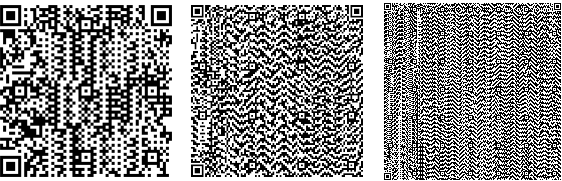
\includegraphics[width=9cm]{QRCodes.png}
\caption{QR code versions 10, 20, and 40 respectively.}
\end{figure}

\section{My Progress}
\subsection{Infrastructure} 
I will give a brief overview of how my infrasture is set up and explain the advantages of the technologies I have chosen. My current infrastructure involves three servers that are all running Ubuntu 14.04. The first server is used as the Kerberos key distribution center (KDC) running version 5 and a domain name server that uses Bind version 9 \cite{Bind}, the second server hosts an Apache web server which can be only be accessed with a valid Kerberos ticket from the KDC server. At the moment the Apache server is playing the role of any possible future Kerberos enabled service. It is a good service to use when testing because there is instant visual feedback when it is working. A use case that results in me being able to access the Apache server could be replaced with any other service such as SSH or access to my account from the login GUI.

I am using Kerberos because it is runs on all popular operating systems and has built in support in a lot of existing services such as Apache, SSH, and Samba. This means that when a service is configured to connect with the user's KDC, they can use their TGT to access restricted web pages, ssh into protected machines, and access specific folders. I am using Kerberos version 5 because it is the most recent and has resolved some security concerns that were present in version 4 \cite{KerbUpdate}. Kerberos is also useful because all tickets have an expiry time. This is important in my system because if a man in the middle attack is performed, then the attacker can only abuse the until it expires. Kerberos is single sign on which is useful in our QR code based system because the user does not have to enter their username and password for each individual service they are trying to access. It is a protocol that is supported on all major operating systems and is well tested. If I was to try and design an authentication protocol myself it would require me to do all of the integration and testing which would take a long time without providing very much benefit.

In my project QR codes are going to be used as a primary communication channel between the user and their services. QR codes are a good option because they are easy to use, and hard to perform a man in the middle attack on. The malicious user would have to get a copy of all the user's QR codes before they could use them themselves.

Unfortunately QR codes do not have support direct binary encoding, this means that Kerberos tickets (which are stored in binary) need to be converted to an alphanumeric format before being encoded. I am currently converting the tickets to hex but in the future I will convert them to base64 because it makes more use of the alphanumeric character set, allowing QR code sizes to be reduced further.

\subsection{Dynamic Grouping of Users}
Dynamic grouping of users is a concept which is used in two of my use cases. The idea is that a Kerberos enabled network has a set of groups with exclusive access to particular resources. A user needs to be a member of the group controling the resources before they are given access. Groups can be long lasting, but in my use cases I have designed them to be set up for short term interactions where users are given access to some resources for short periods to furfull a particular goal such as collaboration. At the end of the interaction e.g. working day or meeting, the group is cleared so that each time that group is used it has a fresh start and prevents users from accessing the resources outside of the intended times. Users are added to the group when they meet certain conditions e.g.\ they are in the meeting. Kerberos lacks native group control, so needs to be implemented by the service using Kerberos. My proposed system puts group support into Kerberos, then uses that to control when users can access particular resources. By having group support directly in Kerberos it creates a single point that needs to be changed, rather than having each resource controlling its own group independently.
%need to mention that there is no build in support for Kerberos groups at the moment

The idea of a dynamic group is that the user must perform an action which will get them added to the group, once they are in the group they have access to that groups resources, but will lose them again once they leave the group. How a user is added to a group can be done a number of different ways that I will go into shortly. Groups can be set up for meetings so that the users can access shared resources for the duration of the meeting, or could be used to ensure that the user can only log into a computer if they are in the room. By having these restrictions there is reduced risk of the users account, or resources being abused by a malicious user.

There are many ways of saying if a user is in the room or not, all are fit for different situations. The three main ways considered are: locating the user with Wi-Fi, GPS, and scanning of QR codes which will come in two forms; codes scanned an admin, and codes scanned by the user.
\begin{itemize}

\item Wi-Fi: It is possible to triangulate a user’s position using multiple Wi-Fi routers. As long as the user is connected to the systems Wi-Fi then their position can be worked out within X meters, which means that the system would be able to detect which room a user is in. The problem with this system is that it requires Kerberos to be integrated with the routers. It also means there needs to be a database of MAC addresses so that when a device is in range, the right user is associated with it. This means that a MAC address could be spoofed but the malicious user would have to spoof the MAC address, be in the right location, and have the victim users QR code tickets. This would be good for situations where a user needs to be confirmed to be in a room that does not need any kind of supervision.

\item GPS: GPS would would similar to Wi-Fi. The signal would have to be coming from a smartphone, and there would need to be a way of telling who was sending which GPS signal and it can happen automatically. It is not accurate indoors, so cannot be used to identify if a user is in a particular room. Another problem is that GPS can be easily spoofed, to be sure that the signal is correct, users of the system would need to be issued a GPS tracker which would syncronize directly with the KDC. By using the tracker the KDC knows it can trust the signal coming from it.

\item QR Code - User Scanned: When we need the user to prove they are in a particular room we can have them scan a room specific QR code which they scan after they have acquired their Kerberos ticket. The room specific code is combined with their ticket so that the the resource they are scanning their code at can see that they have both the rooms code and their ticket. This can be spoofable but if the room codes are changed enough then risk that they will be misused can be reduced.

\item QR Code - Admin Scanned: Used when access is being given to high value resources. The only way a user can get access to these is through the admin scanning their QR code. The idea is that these are often used for short term meetings where access to the resources is as limited as possible. The benefit of the admin having to scan the code also means that a meeting can take place with the admin being selective about who is given access rights to the meetings resources.

\end{itemize}


\subsection{Optimisation of QR Codes}


\subsection{Transfer of a Login Session Use Case}
%TODO: Change to a footnote
I am going to give a run through of my basic use case to show how a user’s ticket can be transferred from one machine to another using QR codes \cite{YouTubeDemo}. Though basic, this use case shows that it is possible for a Kerberos ticket to be transferred between machines using QR codes. In the demo for this use case the QR codes are displayed on the computer screen, but an implemented version of this with a phone could display those QR codes on the phones screen to have the same effect. The process of this use case is outlined below:

\begin{itemize}
	\item Both computer A and B have no Kerberos tickets, and therefore are unable to access the Apache server.
	\item Computer A runs kinit which is a command line program used to authenticate a user to the Kerberos KDC and get their TGT. They enter their details and are given their TGT. They can then use this ticket to negotiate a ticket for the Apache server, granting them access to its resources.
	\item Computer A then runs the QR code creating program. The program takes the TGT from the ticket cache (the location Kerberos tickets are stored) and converts it to hex, it then takes the hex and splits it into small sections. Each of those sections are then encoded into a QR code with a number used to identify the order of the QR codes so they can be reassembled. 
	\item Computer B, which is running the QR code scanning software, scans each of the QR codes created by Computer A. When all the codes are decoded they are reassembled using the ordering numbers from before, converted back to binary, and then added to the Kerberos ticket cache. Computer B is now able to use the TGT just as Computer A could before to negotiate a ticket to access the Apache server.
	\item The tickets from computer A have now been transferred solely using QR codes as the primary means of communication.
\end{itemize}

If this was created, the use case would be carried out in a very similar way, but with computer A being replaced with an Android smartphone. The user would enter their login details into their phone which would create the QR codes for them to scan at any of the accepting systems, authenticating themselves to that system.

\subsection{Meeting Room Use Case}
In this use case, there is a meeting room with particular resources that users in the meeting need to access. Access should be easy for those in the meeting, but difficult for those outside of the meeting. Users get access to the resources such as a shared file system and printer server by being in the meeting room group. Each meeting has an admin who scans users Kerberos ticket QR codes as they enter. When a user enters or leaves the meeting room their QR codes are scanned to show this transition, and as a result they will be added or removed from the meeting room group. Users within the meeting can use the shared resources to collaborate from any of their Kerberos enabled devices. A malicious user in this use case would need to be physically present in the room. Kerberos tickets for these resources have a short lifespan, but can be renewed without a password prompt until the end of meeting. This means users in the room will be able to collaborate for the entire duration without reentering their password, but their device will have to keep renewing their ticket from KDC. Each time the ticket is renewed the KDC will check to see that the user is still part of the meeting group, if they are not then it will simply not give them the ticket they need for the resources, preventing the user from accessing them furthur.

Having Kerberos manage the users in the group means that the admin only needs to send the update to a single place. By doing it all in Kerberos also means that the users do not need access to the internet, only to the KDC.

\subsection{Proximity to Resources}
We want our users to only be able to use resources if they are actually in the geographical area of the computers. The phones GPS can be used to show were a user is, and such can be used to tell the KDC when the user is in or near the building with the resources. Users in the area are kept in a dynamic group so the KDC has an easy way of checking who should be getting tickets. This use case works in a very similar way to the meeting room, but rather than entering the particular room they are entering a certain proximity to the department. Since it is done with GPS is also means it can be done automatically. Since the users phone is tied to the KDC, it means that the KDC could inform the user that someone is attempting to access their account while they are out of the area. The problem with this use case is that the users GPS can not always be trusted, some versions of Android built around privacy are made to send incorrect GPS signals. To remedy this users can have a trusted device with them for the sole purpose of reporting their GPS signal. This means we can trust the GPS signal we are getting, but does also mean an increase in cost to the user.


%This use case would use a dynamic group of users to say who has currently been in the lab, or who is in the lab at this moment in time. It works similar to the meeting room use case, but the focus here is the protection of the users account. The lab has a QR code which is the encoded nonce for that day, when the user enters the lab they scan that QR code with the Android application. The application encrypts the users ID with the days nonce from the scanned QR code then sends that message to the KDC. The KDC attempts to decrypt the message with the days nonuce, if successful it will add that user to lab dynamic group for the rest of the day. A user has to be in this group before they are able to get the principle required to log into the labs computers. The user group is reset at the beginning of each day. By putting this measure in place it means that a users account details, and their phone must be compromised before a malicious user can access their account. Attempts to access an account which has not verified its presence for the day can be flagged to reduce the effectiveness of bruteforce password guessing.


\section{Related Work}
\subsection {Web Authentication Using A Mobile Phone}
This is a method of authentication using a mobile phone, but rather than using a QR code to authenticate the user it puts a proxy between the user and an untrusted computer they need to use \cite{MobileRelated}. The proxy server stores the usernames and passwords. A text message is used to authenticate the user's session to the proxy, and the proxy acquires the login sessions for the user so they do not have to enter usernames and passwords on the suspicious computer.

My solution takes a different approach to this one, theirs can run on any computer because they just need to connect to their secure proxy. I sacrifice the ability to work anywhere for allowing more uses than just the web, and users of my program can transfer their permissions from one computer to another without having to enter their username and password again. 

\subsection{QR Code Based Door Access}
This project uses QR codes to open doors \cite{QRRelated}. The QR code does not expire which is dangerous, but it seems the main purpose of the project is for convenience over security. The idea behind their project is that a user can be emailed their access codes and seem intended to replace key cards. The problem with this method is that replay attacks could be set up to copy a user's QR code and give it to the attacker.

My implementation differs from this because rather than storing an access key, the QR codes in my system store the TGT which could be used to get the user a login session at a computer as well as room access. Their system sends QR codes via email. If someone was able to perform a man in the middle on their mailserver they could gain access to every QR code emailed out.


\section{Results}
Here I'm going to show the output of my programs. The output looks very similar to how the sequence diagrams look, with each action generating a line saying what it is doing. After looking at the results I will then explain how this improves on a use case that does not have access to my application.

\subsection{Meeting Room Results}
The above is an executed version of the use case using the proof of concept programs I have made. The user starts outside of the meeting room, they try and get their ticket, and the ticket check fails and the ticket is deleted. Next it is similated that they enter the room by scanning their QR code, they are then put into the meeting room group. When they try to get their ticket next it the check passes, allowing them to keep their ticket. They then use this ticket to SSH into the printer and the fileserver. SSH in this case takes to place of the two Kerberos enabled services, in the real version the user would actually check that they can print and access the file server. The user then leaves the room, when the user tries to refresh their ticket the KDC sees that they are no longer in the room and removes their ticket.

\subsection{Daily Room Access Results}
Here is an example version of the Daily Room Access use case. The user attempts to log into their machine, but cannot until they have been added to the lab group by scanning their QR code. Once the code has been scanned the user is added to the lab group and can begin accessing the lab machines. I use SSH to show the users ability to log into the computer. This proof of concept works very similar to how the meeting room use case works





\section{Problems Encountered}
Parts of the project did not go as planned. Overall this did not limit the knowledge that was gained from the project, does limit the useable applications created by the project. Before work could be started on the project I needed to set up the Kerberos infrastruture. My unfamiliarity with it meant that it took longer than expected, but a lot was learnt about Kerberos and how it would fit into the scope of the project. After better researching the Android application it was deceided that it was better of to implement a proof of concept rather than creating an actual application. This is because it made testing much faster as everything was contained within virtual machines, and it also meant that different use cases could be quickly prototyped using command line programs without having to worry about creating a GUI on an unfamiliar platform.

My checks to see if a ticket was valid all had to be client side. This is not optimal in a real system because it allows a malicious user to take their valid ticket before the check has taken place. Since my proof of concept assumes a non-malicious user it has not been a problem for my tests. Work on integrating it into MIT Kerberos would take a long time since it is a very large code base, so for my project I felt that showing how the system would work if implemented was enough.



% Probably not needed anymore but handy for referencing 
\section{Future Work}
A big part of my project is coming up with ways the QR codes can be used and then implementing them. We have come up with some potential use cases, and this semester I am working out the specifics involved in the use cases and implementing them. I’m going to go through some of my considered use cases and work out any of the details. I also need to implement the Android application so that these use cases can be carried out in a portable manner.

\subsection{Android Application}
In my proof of concept I have shown what my system is capable of doing, but in the future I want the user to be able to start the interaction with an Android smartphone. The reason Android is the target platform is because MIT Kerberos has been ported to it \cite{KerbDroid}. There is also an open source application I can use as a reference on how to build my own Kerberos application \cite{KerbApp}. My use cases should have low processing requirements so even modest processors will be able to run my application. Smartphones also come with cameras, Wi-Fi, and displays built in. This means that my use cases can include the user connecting to the internet, scanning QR codes with their camera, or displaying QR codes on their screen without fear that user will not have the hardware to perform these actions.

\subsection{Collaboration On A LAN}
In the future I want to be able to use the Android application as a means of establishing trust between a group collaborating on a LAN. The master user could create a QR code which can be scanned by all the other users. They use the information in this QR code to set up a trust relationship between their own KDC and the KDC of the LAN they are collaborating on. Once this trust is set up, each of the users can use their own Kerberos account to access services on the network they are collaborating on without having to get their own account for the LAN. It also means that the owner of the LAN’s KDC can discontinue the trust with any KDCs of users leaving the LAN. With this use case there is potential for a user to cause damage to any services they are give access rights to, but the user who caused the damage will be known because they must use their own account, and the trust can be broken with them at anytime, stopping their access.

\subsection{Transferring A Login Session}
I also want to allow a user to take their login session elsewhere using their phone. The idea is that if a user has already logged in then they should be able to take that session with them on their phone and continue it on the same network without entering their details again. Upon logout the user has the option to receive QR codes for their phone which contains their TGT. They can scan the QR codes from their phone at any other computer on the network running my QR code scanning program and it will place their TGT into the ticket cache and log them in without them having to enter their details. For this use case to operate correctly I need to be able have my program as part of the login GUI. Possible threats with this use case are that a user could be out of the room and have a malicious user come and “steal” their login session, this is something I will need to consider when making the program.

\begin{thebibliography}{9}
\bibitem{Bind} Douglas B. Terry, Mark Painter, David W. Riggle Songnian Zhou, The Berkeley Internet Name Domain Server, 1984.   
\bibitem{Kerb} B. Clifford Neuman, Theodore Ts'o, Kerberos: An Authentication Service for Computer Networks, 1994. 
\bibitem{QR} Needed.
\bibitem{KerbDroid} krb5-anonsvn, https://github.com/cconlon/krb5-anonsvn, 2014.
\bibitem{KerbApp} kerberos-android-ndk, https://github.com/cconlon/kerberos-android-ndk, 2014.
\bibitem{KerbUpdate} Kerberos Version 4 End of Life Announcement, http://web.mit.edu/kerberos/krb4-end-of-life.html, 2014.
\bibitem{MobileRelated} Secure Web Authentication with Mobile Phones, http://homepages.mcs.vuw.ac.nz/~ian/shared/papers/secureweb.pdf, 2014.
\bibitem{QRRelated} LibeTech QR Code Door Lock, http://www.jeremyblum.com/portfolio/libetech/, 2014.
\bibitem{YouTubeDemo} QR Code Proof of Concept, https://www.youtube.com/watch?v=v8ZZWC-jXeM\&list=UU3CfgH3Wtm0TTpxq0I92XFw, 2014.
\end{thebibliography}
\end{document}